\chapter{Riemann Sums}

\section{The Meaning of the Area Under a Function}

Let's look at the example of a hammer tossed in the air from a previous chapter. As you may recall, if a hammer is tossed up from the ground at 5 m/s, its velocity can be described as $v(t) = 5-9.8t$ (on Earth, where the acceleration due to gravity is approximately $-9.8$ $\frac{m}{s^2}$). The velocity function of our hammer from when it is tossed ($t=0$) to when it hits the ground $t\approx1.02$) is shown in figure \ref{fig:hammer}.

\begin{figure}[htbp]
	\centering
	\begin{tikzpicture}
		\begin{axis}[axis lines = center, xmin=0, xmax=1.02, xlabel=$t$(sec), ymin=-5, ymax=5, ylabel=$v$(m/s)]
		\addplot[blue, smooth, samples=50]{5-9.8*x};
		\end{axis}
	\end{tikzpicture}
	\caption{Velocity of a hammer thrown upwards at 5 m/s}
	\label{fig:hammer}
\end{figure}

Now, suppose we only have this velocity function and we want to know how high above its initial position the hammer is tossed. Examine the graph: at approximately what time does the hammer reach its peak height? (Hint: what should the hammer's velocity be when it reaches its peak?). At the highest point of its flight, the hammer's velocity will be $0$ $\frac{m}{s}$, which occurs at approximately $t=0.5s$ (it's actually $t=0.5102s$ but we don't need to be that precise for this example). 

Now that we know \textit{when} the hammer reaches its peak, how can we determine \textit{how high} that peak is? Recall that velocity is the slope of the position-time graph. Since slope is change in position divided by change in time (in this case, as time is on the $x$-axis and position on the $y$-axis), then the slope must have units of [position]/[time] which could be $\frac{m}{s}$, $\frac{miles}{hr}$, etc. These are units of velocity! 

In figure \ref{fig:hammer}, you can see that the units on the $x$-axis are seconds and on the $y$-axis the units are $\frac{m}{s}$. If we are looking for a \textit{displacement} (that is, how far from its initial position the hammer has traveled), we are looking for a solution with units of meters. To yield an answer with those units, we wouldn't use the slope of the graph: this would yield an answer with units $\frac{m}{s^s}$, the units for acceleration. Instead, we need to \textit{multiply}! The area between the velocity function and the $x$-axis (see figure \ref{fig:hammerarea}) can be found this way:

$$Area=\frac{1}{2}bh$$where b is the base of the triangle and h is the height. 
$$Area=\frac{1}{2}(0.5s)(5\frac{m}{s})$$
$$Area=1.25m$$


\begin{figure}[htbp]
	\centering
	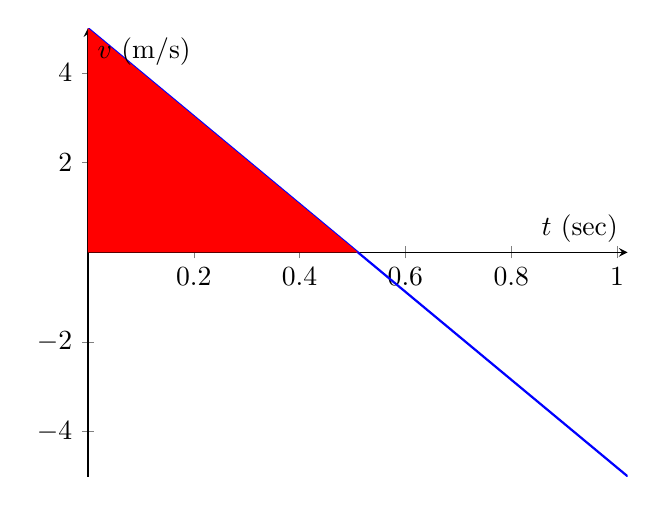
\begin{tikzpicture}
		\begin{axis}[axis lines = center, xmin=0, xmax=1.02, xlabel=$t$ (sec), ymin=-5, ymax=5, ylabel=$v$ (m/s)]
		\addplot[blue, smooth, thick, samples=50]{5-9.8*x};
		\coordinate (c0) at (0,0);
		\coordinate (c1) at (0.5102, 0);
		\coordinate (c2) at (0, 5);
		\fill[red] (c0) -- (c1) -- (c2) -- cycle;
		\end{axis}
	\end{tikzpicture}
	\caption{The area under $v(t)$ from $x=0$ to $x=0.5$ is equal to the displacement of the hammer}
	\label{fig:hammerarea}
\end{figure}

Notice that when multiplying the change in time ($0.5$ $s$) by the change in velocity ($1.25$ $\frac{m}{s}$), the seconds units cancel, yielding a result with units of meters. Therefore, the hammer reaches a peak height of $\approx1.25$ $m$, which you can confirm by examining the graph originally presented for the hammer toss in the chapter on graph shape.

\subsection{Determining the Meaning of the Area with Units}
%brief explanation, justification, real-world etc., with one more example

\begin{Exercise}[label=units1]
What units will the area shown in the graph have? Based on your answer, does the area represent a displacement, a net change in velocity, or a net change in acceleration?\\
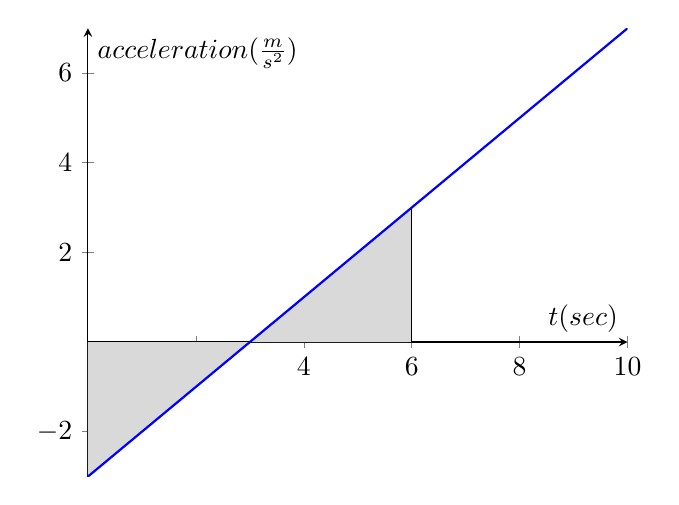
\begin{tikzpicture}
		\begin{axis}
		[axis lines = center, xmin=0, xmax=10, ymin=-3, ymax=7, xlabel=$t(sec)$, ylabel=$acceleration(\frac{m}{s^2})$]
		\fill[gray!30](0,-3)--(3,0)--(0,0)--cycle;
            \fill[gray!30](3,0) -- (6,0) -- (6, 3)--cycle;
            \addplot[black,very thin]coordinates{(6,0) (6, 3)};
		\addplot[blue, thick, samples=50, domain=0:10]{x-3};
		\end{axis}
	\end{tikzpicture}  
\end{Exercise}

\begin{Answer}[ref=units1]
The units on the $x$-axis are $s$ and the units on the $y$-axis are $\frac{m}{s^2}$. The area then would have units of $s \times \frac{m}{s^2}=\frac{m}{s}$. Based on the units, the area represents a net change in velocity. 
\end{Answer}

\begin{Exercise}[label=units2]
	The graph below shows historical data of the number of deaths due to SARS in Singapore over several months in 2003. What would the area under the curve represent?\\
	
	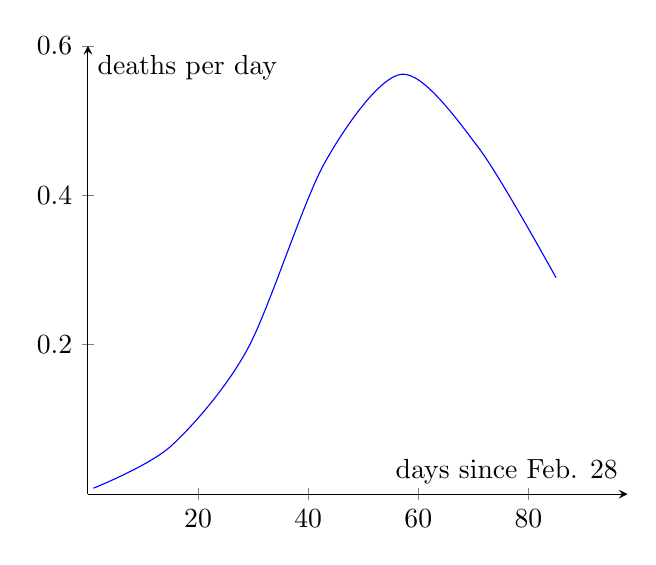
\begin{tikzpicture}
		\begin{axis}[axis lines = center, xmin=0, xmax=98, ymin=0, ymax=0.6, xlabel=days since Feb. 28, ylabel=deaths per day]
		\addplot[blue, smooth]coordinates{(1, 0.0079) (15, 0.0638) (29, 0.1944) (43, 0.4435) (57, 0.5620) (71, 0.4630) (85, 0.2897)};
		\end{axis}
	\end{tikzpicture}
\end{Exercise}

\begin{Answer}[ref=units2]
	The units of the area will be $days \times \frac{deaths}{day}=deaths$. The area under the curve represents the total number of people who died of SARS in Singapore during the time period represented [from March 1 to May 24 (if you took the time to do the math for the dates)]. 
\end{Answer}

\begin{Exercise}[label=units3]
	Oil leaked from a tank at a rate of $r(t)$ liters per hour. A site engineer recorded the leak rate over a period of 10 hours, shown in the table. Plot the data. How could you estimate the total volume of oil lost?\\
	\begin{tabular}{c|c|c|c|c|c|c}
	$t(\text{h})$ & 0 & 2 & 4 & 6 & 8 & 10 \\
	$r(t)(\text{L/h})$ & 8.7 & 7.6 & 6.8 & 6.2 & 5.7 & 5.3 \\
	\end{tabular}
\end{Exercise}

\begin{Answer}[ref=units3]
	\begin{tikzpicture}
		\begin{axis}[axis lines = center, xmin=0, xmax=10, ymin=0, ymax=10, xlabel=$t$(h), ylabel=$r(t)$(L/h)]
		\addplot[blue, mark=*, dashed]coordinates{(0, 8.7) (2, 7.6) (4, 6.8) (6, 6.2) (8, 5.7) (10, 5.3)};
		\end{axis}
	\end{tikzpicture}
	\\
	Based on the units, the area under the data would represent the total oil lost. One way to estimate this area would be to create rectangles, but there are other valid methods. 
\end{Answer}

\section{Estimating the area under functions}

In the hammer example above, it was easy to determine the area under the function, since the area took the shape of a triangle. But what about finding the area under a more complex function, such as $f(x) = sin{x}+x$ (shown in figure \ref{fig:riemannsine})?

\begin{figure}[htbp]
	\centering
	\begin{tikzpicture}
		\begin{axis}
            [axis lines = center, 
            xmin=0, xmax=3.141592, xlabel=$x$, xtick={0, 0.785398, 1.570796, 2.356194, 3.141593}, xticklabels={$0$, $\frac{\pi}{4}$, $\frac{\pi}{2}$, $\frac{3\pi}{4}$, $\pi$},
            ylabel=$y$, ymin =0, ymax=3.25, ytick={1, 2, 3}, yticklabels={$1$, $2$, $3$}]
			\addplot[blue, samples=50, domain=0:3.141592]{sin(deg(x))+x};
		\end{axis}
	\end{tikzpicture}
	\caption{$f(x) = \sin{x}+x$}
	\label{fig:riemannsine}
\end{figure}

How can we determine the area under $f(x) = \sin{x}+x$ from $x=0$ to $x=\pi$? We can \textit{estimate} the area of that region by dividing the region into rectangles, finding the areas of the rectangles, and adding the areas. As an example, we will divide the region under $f(x) = \sin{x}+x$ into 4 intervals, shown in figure \ref{fig:sinesections}.

\begin{figure}[htbp]
	\centering
	\begin{tikzpicture}
		\begin{axis}[axis lines = center, 
            xmin=0, xmax=3.15, xlabel=$x$, xtick={0, 0.785398, 1.570796, 2.356194, 3.141593}, xticklabels={$0$, $\frac{\pi}{4}$, $\frac{\pi}{2}$, $\frac{3\pi}{4}$, $\pi$},
            ylabel=$y$, ymin =0, ymax=3.25, ytick={1, 2, 3}, yticklabels={$1$, $2$, $3$}]
			\addplot[blue, thick, samples=50, domain=0:6.283185]{sin(deg(x))+x};
                \addplot[black, samples=50]coordinates{(0.785, 0) (0.785, 1.4925)};
                \addplot[black, samples=50]coordinates{(1.570796, 0) (1.570796, 2.5708)};
                \addplot[black, samples=50]coordinates{(2.356194, 0) (2.356194, 3.0633)};
                \addplot[black, samples=50]coordinates{(3.141592, 0) (3.141592, 3.141592)};
		\end{axis}
	\end{tikzpicture}
	\caption{$f(x) = \sin{x}+x$ divided into 4 regions}
	\label{fig:sinesections}
\end{figure}

As you can see in figure \ref{fig:sinesections}, each rectangle will have a width of $\frac{\pi}{4}$. But what about the height? One way is to use the value of the function at the rightmost value of each rectangle, as shown in figure \ref{fig:sineright}. 

\begin{figure}[htbp]
	\centering
	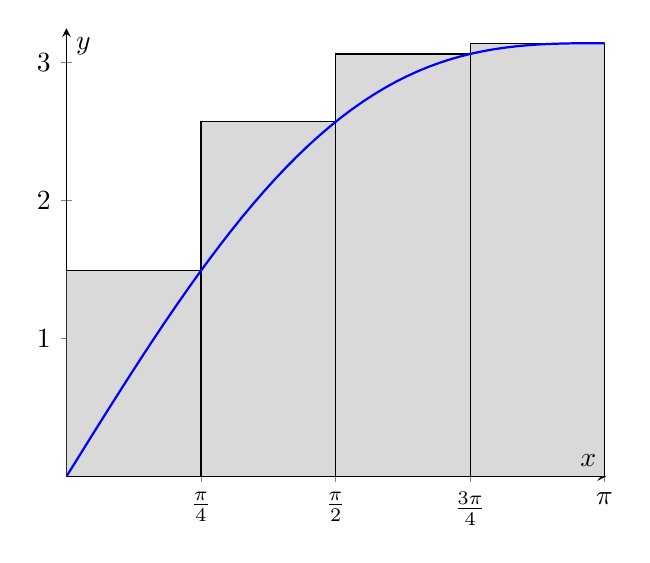
\begin{tikzpicture}
		\begin{axis}[axis lines = center, 
            xmin=0, xmax=3.15, xlabel=$x$, xtick={0, 0.785398, 1.570796, 2.356194, 3.141593}, xticklabels={$0$, $\frac{\pi}{4}$, $\frac{\pi}{2}$, $\frac{3\pi}{4}$, $\pi$},
            ylabel=$y$, ymin =0, ymax=3.25, ytick={1, 2, 3}, yticklabels={$1$, $2$, $3$}]
                \filldraw[fill=gray!30] (0,0) rectangle (0.785, 1.4925);
                \filldraw[fill=gray!30] (0.785398, 0) rectangle (1.570796, 2.5708);
                \filldraw[fill=gray!30] (1.570796, 0) rectangle (2.356194, 3.0633);
                \filldraw[fill=gray!30] (2.356194, 0) rectangle (3.141592, 3.141592);
			\addplot[blue, thick, samples=50, domain=0:3.141592]{sin(deg(x))+x};
		\end{axis}
	\end{tikzpicture}
	\caption{Four rectangle sections with heights determined by rightmost value of $f(x)$ on each interval}
	\label{fig:sineright}
\end{figure}

We can easily calculate the areas of each of these rectangles:
$$\frac{\pi}{4} \times f(\frac{\pi}{4}) + \frac{\pi}{4} \times f(\frac{\pi}{2}) + \frac{\pi}{4} \times  f(\frac{3\pi}{4}) + \frac{\pi}{4} \times f(\pi)$$
$$\approx \frac{\pi}{4} \times (1.4925 + 2.5708 + 3.0633 + 3.1416) = 8.0646$$

Based on figure \ref{fig:sineright}, will the calculated area be an overestimate or an underestimate? Each of the rectangles overshoots the function, so this will be an overestimate. What about using the leftmost value of $f(x)$ of each interval to determine the height of the rectangles? This is shown in figure \ref{fig:sineleft}.

\begin{figure}[htbp]
	\centering
	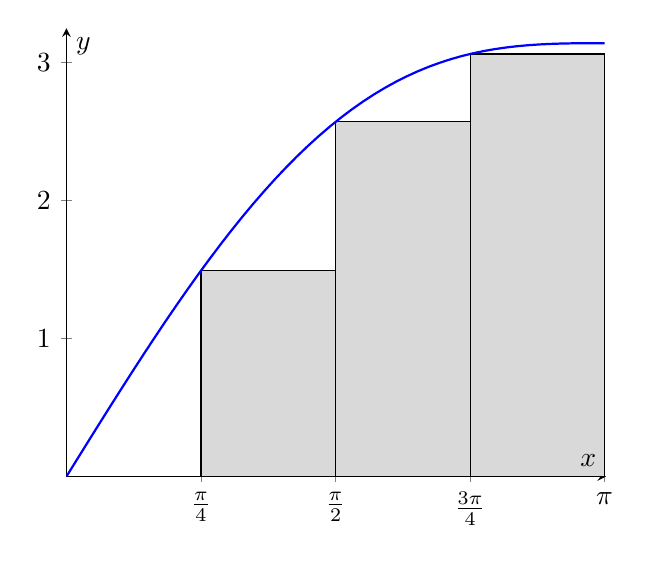
\begin{tikzpicture}
		\begin{axis}[axis lines = center, 
            xmin=0, xmax=3.15, xlabel=$x$, xtick={0, 0.785398, 1.570796, 2.356194, 3.141593}, xticklabels={$0$, $\frac{\pi}{4}$, $\frac{\pi}{2}$, $\frac{3\pi}{4}$, $\pi$},
            ylabel=$y$, ymin =0, ymax=3.25, ytick={1, 2, 3}, yticklabels={$1$, $2$, $3$}]
                \filldraw[fill=gray!30] (0,0) rectangle (0.785, 0);
                \filldraw[fill=gray!30] (0.785398, 0) rectangle (1.570796, 1.4925);
                \filldraw[fill=gray!30] (1.570796, 0) rectangle (2.356194, 2.5708);
                \filldraw[fill=gray!30] (2.356194, 0) rectangle (3.141592, 3.0633);
			\addplot[blue, thick, samples=50, domain=0:3.141592]{sin(deg(x))+x};
		\end{axis}
	\end{tikzpicture}
	\caption{Four rectangle sections with heights determined by leftmost value of $f(x)$ on each interval}
	\label{fig:sineleft}
\end{figure}

Notice that because $f(0)=0$, the height of the first rectangle is zero, so we don't see it on the graph. To find the area of these rectangles:
$$\frac{\pi}{4} \times f(0) + \frac{\pi}{4} \times f(\frac{\pi}{4}) + \frac{\pi}{4} \times f(\frac{\pi}{2}) + \frac{\pi}{4} \times f(\frac{3\pi}{4})$$
$$\approx \frac{\pi}{4} \times (0 + 1.4925 + 2.5708 + 3.0633)=5.5972$$

This is an underestimate. Therefore, the true value of the area under $f(x) = \sin{x} +x$ is between $5.5972$ and $8.0646$. This is an awfully wide window! We can narrow our estimate by increasing the number of intervals. Graphs of $f(x)$ with 10 intervals are shown in figure \ref{fig:tenintervals}.

\begin{figure}
	\centering
	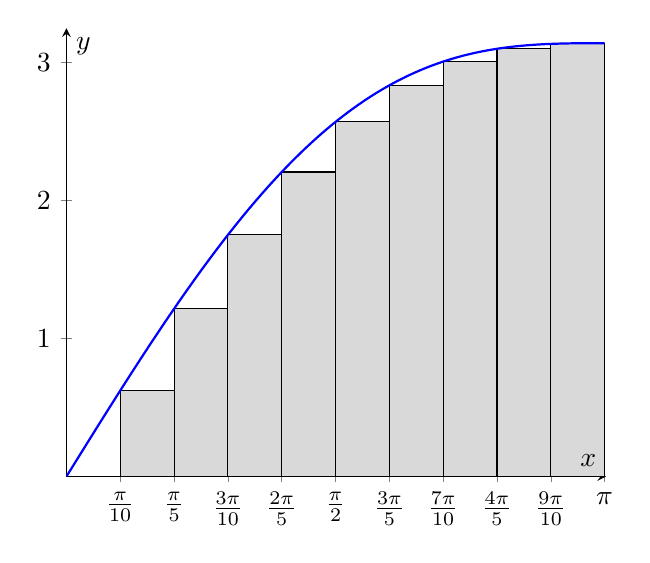
\begin{tikzpicture}
		\begin{axis}
		[axis lines = center, 
		xmin=0, xmax=3.15, xlabel=$x$,
		xtick={0, 0.31416, 0.62832, 0.94248, 1.25664, 1.57080, 1.88496, 2.19911, 2.51327, 2.82743, 3.14159}, 
		xticklabels={$0$, $\frac{\pi}{10}$, $\frac{\pi}{5}$, $\frac{3\pi}{10}$, $\frac{2\pi}{5}$, $\frac{\pi}{2}$, $\frac{3\pi}{5}$, $\frac{7\pi}{10}$, $\frac{4\pi}{5}$, $\frac{9\pi}{10}$, $\pi$}, 
		ymin=0, ymax=3.25, ylabel=$y$,
		ytick={1, 2, 3},
		yticklabels={$1$, $2$, $3$}]
			\filldraw[fill=gray!30, draw=black](0,0) rectangle (0.31416, 0);
			\filldraw[fill=gray!30, draw=black](0.31416, 0) rectangle (0.62832, 0.62318);
			\filldraw[fill=gray!30, draw=black](0.62832, 0) rectangle (0.94248, 1.2161);
			\filldraw[fill=gray!30, draw=black](0.94248, 0) rectangle (1.25664, 1.75149);
			\filldraw[fill=gray!30, draw=black](1.25664, 0) rectangle (1.57080, 2.20769);
			\filldraw[fill=gray!30, draw=black](1.57080, 0) rectangle (1.88496, 2.5708);
			\filldraw[fill=gray!30, draw=black](1.88496, 0) rectangle (2.19911, 2.83601);
			\filldraw[fill=gray!30, draw=black](2.19911, 0) rectangle (2.51327, 3.00813);
			\filldraw[fill=gray!30, draw=black](2.51327, 0) rectangle (2.82743, 3.10106);
			\filldraw[fill=gray!30, draw=black](2.82743, 0) rectangle (3.14159, 3.13645);
			\addplot[blue, thick, samples=100, domain=0:3.141592]{sin(deg(x))+x};
		\end{axis}
	\end{tikzpicture}
	
	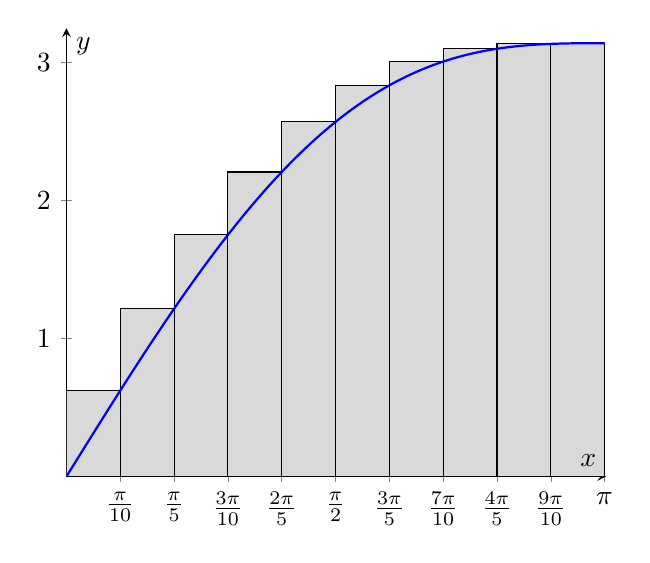
\begin{tikzpicture}
	\begin{axis}
		[axis lines = center, 
		xmin=0, xmax=3.15, xlabel=$x$,
		xtick={0, 0.31416, 0.62832, 0.94248, 1.25664, 1.57080, 1.88496, 2.19911, 2.51327, 2.82743, 3.14159}, 
		xticklabels={$0$, $\frac{\pi}{10}$, $\frac{\pi}{5}$, $\frac{3\pi}{10}$, $\frac{2\pi}{5}$, $\frac{\pi}{2}$, $\frac{3\pi}{5}$, $\frac{7\pi}{10}$, $\frac{4\pi}{5}$, $\frac{9\pi}{10}$, $\pi$}, 
		ymin=0, ymax=3.25, ylabel=$y$,
		ytick={1, 2, 3},
		yticklabels={$1$, $2$, $3$}]
			\filldraw[fill=gray!30, draw=black](0,0) rectangle (0.31416, 0.62318);
			\filldraw[fill=gray!30, draw=black](0.31416, 0) rectangle (0.62832, 1.2161);
			\filldraw[fill=gray!30, draw=black](0.62832, 0) rectangle (0.94248, 1.75149);
			\filldraw[fill=gray!30, draw=black](0.94248, 0) rectangle (1.25664, 2.20769);
			\filldraw[fill=gray!30, draw=black](1.25664, 0) rectangle (1.57080, 2.5708);
			\filldraw[fill=gray!30, draw=black](1.57080, 0) rectangle (1.88496, 2.83601);
			\filldraw[fill=gray!30, draw=black](1.88496, 0) rectangle (2.19911, 3.00813);
			\filldraw[fill=gray!30, draw=black](2.19911, 0) rectangle (2.51327, 3.10106);
			\filldraw[fill=gray!30, draw=black](2.51327, 0) rectangle (2.82743, 3.13645);
			\filldraw[fill=gray!30, draw=black](2.82743, 0) rectangle (3.14159, 3.14159);
			\addplot[blue, thick, samples=100, domain=0:3.141592]{sin(deg(x))+x};
		\end{axis}
	\end{tikzpicture}
	\caption{$\sin{x}+x$ broken into 10 intervals using either the left or right value to determine the height.}
	\label{fig:tenintervals}
\end{figure}

The total area for the left-determined rectangles is $\approx 6.4248$ and for the right-determined is $\approx7.4118$. Therefore, we have narrowed the range for the true area under the curve to $6.4248<A<7.4118$. In general, as you increase the number of intervals, you get closer to the true area. 

For a strictly increasing function, the right sum will be an overestimate and the left sum will be an underestimate of the true area under the curve. In the exercise below, you will examine a strictly decreasing function:

\begin{Exercise}[label=rsum1]
	Estimate the area under the graph of $f(x) = \frac{1}{x}$ from $x=1$ to $x=2$ using four rectangles and right endpoints. Sketch the graph and the rectangles. Is your estimate an overestimate or an underestimate? Repeat using left endpoints. 
	\vspace{100mm}
\end{Exercise}

\begin{Answer}[ref=rsum1]
	Right-determined sum graph:\\
		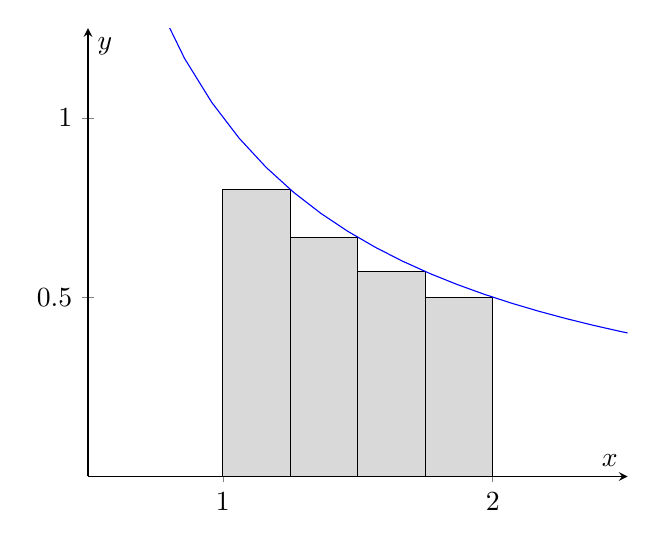
\begin{tikzpicture}
			\begin{axis}
            [axis lines = center, 
            xmin=.5, xmax=2.5, xlabel=$x$, xtick={1, 2}, xticklabels={$1$, $2$},
            ylabel=$y$, ymin =0, ymax=1.25, ytick={0.5, 1}, yticklabels={$0.5$, $1$}]
                \filldraw[fill=gray!30, draw=black](1,0) rectangle (1.25, 0.8);
                \filldraw[fill=gray!30, draw=black](1.25, 0) rectangle (1.5, 0.6667);
                \filldraw[fill=gray!30, draw=black](1.5, 0) rectangle (1.75, 0.5714);
                \filldraw[fill=gray!30, draw=black](1.75, 0) rectangle (2, 0.5);
				\addplot[blue, samples=100]{1/x};
			\end{axis}
		\end{tikzpicture}\\
		The area of the right-determined sum is $0.25\times(0.8+0.6667+0.5714+0.5) = 0.4202$. This is an underestimate of the actual area. \\
	Left-determined sum graph:\\
	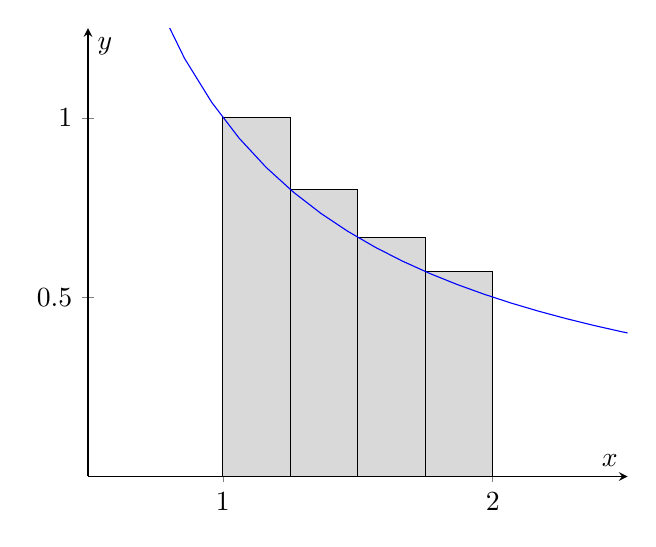
\begin{tikzpicture}
			\begin{axis}
            [axis lines = center, 
            xmin=.5, xmax=2.5, xlabel=$x$, xtick={1, 2}, xticklabels={$1$, $2$},
            ylabel=$y$, ymin =0, ymax=1.25, ytick={0.5, 1}, yticklabels={$0.5$, $1$}]
                \filldraw[fill=gray!30, draw=black](1,0) rectangle (1.25, 1);
                \filldraw[fill=gray!30, draw=black](1.25, 0) rectangle (1.5, 0.8);
                \filldraw[fill=gray!30, draw=black](1.5, 0) rectangle (1.75, 0.6667);
                \filldraw[fill=gray!30, draw=black](1.75, 0) rectangle (2, 0.5714);
				\addplot[blue, samples=100]{1/x};
			\end{axis}
		\end{tikzpicture}	\\
		The area of the left-determined sum is $0.25\times(1+0.8+0.6667+0.5714)=0.7595$. This is an overestimate of the actual area. 
\end{Answer}

You should have found that for the strictly decreasing function $f(x) = \frac{1}{x}$, the right-determined sum is an \textit{underestimate} while the left-determined sum is an \textit{overestimate}. \\


\section{The Riemann Sum}
In the previous section, we estimated the area under functions by dividing the area into approximating rectangles. This method is called a \textit{Riemann Sum}. We will use a general example to formally define the Riemann sum. Consider a generic function divided into strips of equal width (shown in figure \ref{fig:strips}). The width of each strip is $$\Delta x=\frac{b-a}{n}$$ where $a$ is the left endpoint of the interval, $b$ is the right endpoint of the interval, and $n$ is the number of strips. Then the right endpoints of the sections are $$x_1=a+\Delta x$$
$$x_2 = a +2\Delta x$$
$$\ldots \text{ }x_n=a+n\Delta x$$

As above, we can use the value of the function to determine the height of a rectangle whose area approximates the area of the section. (E.g. for the $i^{th}$ strip, the width is $\Delta x$ and the height is $f(x_i)$, see figure \ref{fig:rectangles}). Then the total area approximated by the rectangles is $$R_n = f(x_1)\Delta x + f(x_2)\Delta x + \ldots + f(x_n)\Delta x$$ \\This is the formal definition of the Right Riemann Sum. You can also take a Left Riemann Sum or a Midpoint Riemann Sum, as discussed below. 

\begin{figure}
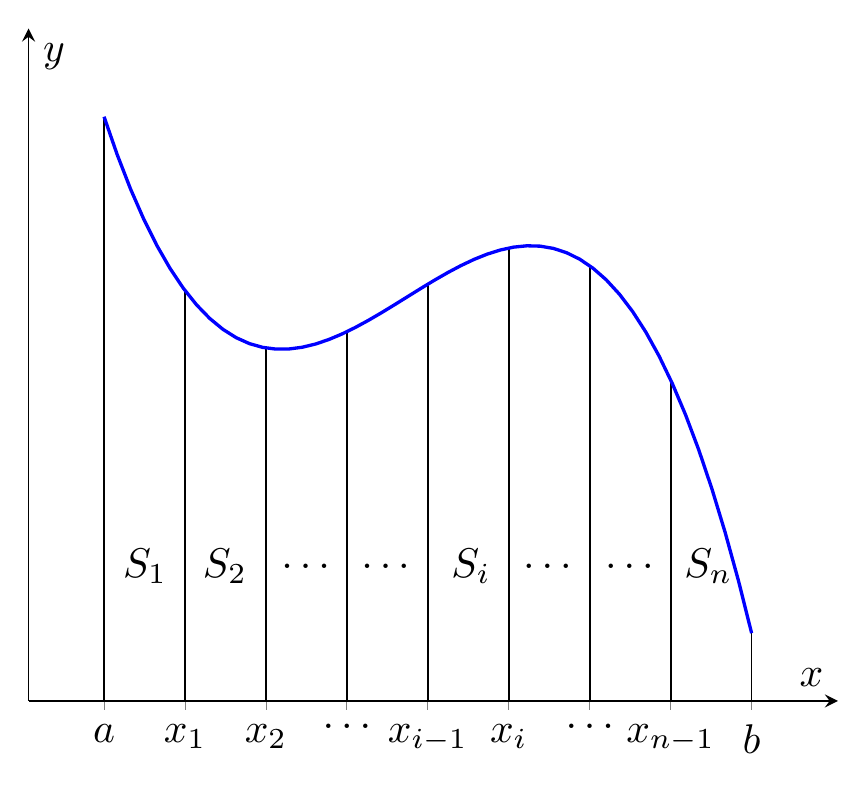
\begin{tikzpicture}[scale=1.5]
	\begin{axis}
	[axis lines=center, 
        xmin = 0.25, xmax = 4, xlabel=$x$, ylabel=$y$, ymin=0, ymax=5, xtick={0.6, 0.975, 1.35, 1.725, 2.1, 2.475, 2.85, 3.225, 3.6}, xticklabels={$a$, $x_1$, $x_2$, $\ldots$, $x_{i-1}$, $x_i$, $\ldots$, $x_{n-1}$, $b$}, ytick=\empty]
        \draw[black] (0.6, 0) -- (0.6, 4.344); %shows a, beginning of interval
        \draw[black] (3.6, 0) -- (3.6, 0.504); %shows b, end of interval
        \draw[black] (0.975, 0) -- (0.975, 3.05189); %end of 1st interval
        \draw[black] (1.35, 0) -- (1.35, 2.62462); %end of 2nd interval
        \draw[black] (1.725, 0) -- (1.725, 2.7458); %end of 3rd interval
        \draw[black] (2.1, 0) -- (2.1, 3.099); %end of 4th interval
        \draw[black] (2.475, 0) -- (2.475, 3.36783); %end of 5th interval
        \draw[black] (2.85, 0) -- (2.85, 3.23588); %end of 6th interval
        \draw[black] (3.225, 0) -- (3.225, 2.38673); %end of 7th interval
        \addplot[blue, thick, samples=50, domain=0.6:3.6]{(1-x)*(x-2)*(x-3)+3}; %function
       	\node[] at (0.79, 1) {$S_1$}; %labeling sections
        \node[] at (1.16, 1) {$S_2$};
        \node[] at (2.3, 1) {$S_i$};
        \node[] at (3.4, 1) {$S_n$};
        \node[] at (1.55,1) {\ldots};
        \node[] at (1.92,1) {\ldots};
        \node[] at (2.67,1) {\ldots};
        \node[] at (3.05,1) {\ldots};
	\end{axis}
\end{tikzpicture}
\caption{A representative function divided into $n$ strips of equal width}
\label{fig:strips}
\end{figure}

\begin{figure}
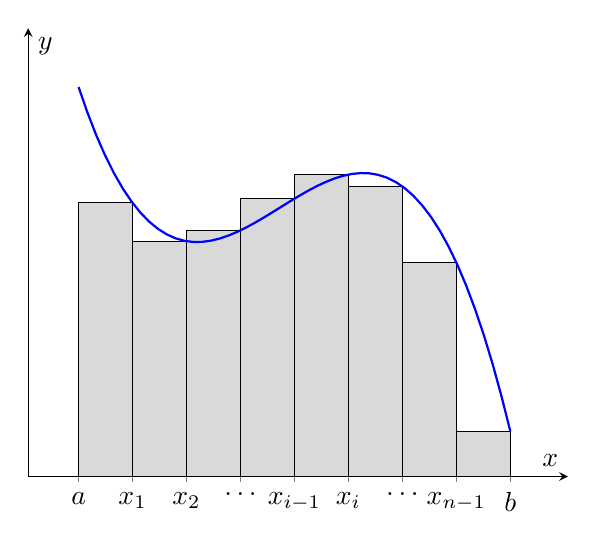
\begin{tikzpicture}
	\begin{axis}
	[axis lines=center, 
        xmin = 0.25, xmax = 4, xlabel=$x$, ylabel=$y$, ymin=0, ymax=5, xtick={0.6, 0.975, 1.35, 1.725, 2.1, 2.475, 2.85, 3.225, 3.6}, xticklabels={$a$, $x_1$, $x_2$, $\ldots$, $x_{i-1}$, $x_i$, $\ldots$, $x_{n-1}$, $b$}, ytick=\empty]
        \filldraw[draw=black, fill=gray!30] (0.6, 0) rectangle (0.975, 3.05189); %1st subinterval
        \filldraw[draw=black, fill=gray!30] (0.975, 0) rectangle (1.35, 2.62462); %2nd subinterval
        \filldraw[draw=black, fill=gray!30] (1.35, 0) rectangle (1.725, 2.7458); %3rd subinterval
        \filldraw[draw=black, fill=gray!30] (1.725, 0) rectangle (2.1, 3.099); %4th subinterval
        \filldraw[draw=black, fill=gray!30] (2.1, 0) rectangle (2.475, 3.36783); %5th subinterval
        \filldraw[draw=black, fill=gray!30] (2.475, 0) rectangle (2.85, 3.23588); %6th subinterval
        \filldraw[draw=black, fill=gray!30] (2.85, 0) rectangle (3.225, 2.38673); %7th subinterval
        \filldraw[draw=black, fill=gray!30] (3.225, 0) rectangle (3.6, 0.504); %8th subinterval
        \addplot[blue, thick, samples=50, domain=0.6:3.6]{(1-x)*(x-2)*(x-3)+3};
	\end{axis}
\end{tikzpicture}
\caption{A representative function divided into $n$ rectangles of equal width, with rectangle height determined by the right endpoint of the subinterval}
\label{fig:rectangles}
\end{figure}

\subsection{Left Riemann Sums}
When taking a left Riemann sum, the height of the rectangle is determined by the value of the function at the lower (left-most) $x$-value. See figure \ref{fig:leftriemann}. We will refer to left Riemann sums as $L_n$, where $n$ is the number of intervals. Then the total area approximated by a Left Riemann sum is is $$L_n = f(x_0)\Delta x + f(x_1)\Delta x + \ldots + f(x_{n-1})\Delta x$$.

\begin{figure}
    \centering
    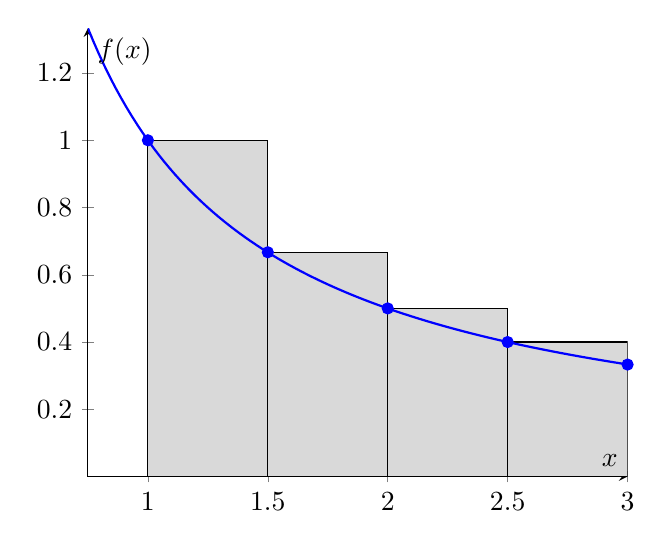
\begin{tikzpicture}
        \begin{axis}[axis lines = center, xmin=0.75, xmax=3, ymin=0, xlabel=$x$, ylabel=$f(x)$]
            \filldraw[fill=gray!30, draw=black] (1,0) rectangle (1.5,1);
            \filldraw[fill=gray!30, draw=black] (1.5,0) rectangle (2, 0.667);
            \filldraw[fill=gray!30, draw=black] (2,0) rectangle (2.5, 0.5);
            \filldraw[fill=gray!30, draw=black] (2.5,0) rectangle (3, 0.4);
            \addplot[blue, thick, samples=100, domain=0.75:3]{1/x};
            \addplot[mark=*, blue, only marks]coordinates{(1,1) (1.5,0.667) (2, 0.5) (2.5,.4) (3,0.333)};
        \end{axis}
    \end{tikzpicture}
    \caption{$L_4$ for $f(x)=\frac{1}{x}$}
    \label{fig:leftriemann}
\end{figure}

\subsection{Right Riemann Sums}
A right Riemann sum uses the right-most value of $f(x)$ to determine the height of the rectangle (an example is shown in figure \ref{fig:rightriemann}). We will refer to the right Riemann sum as $R_n$, where $n$ is the number of intervals.

\begin{figure}
    \centering
    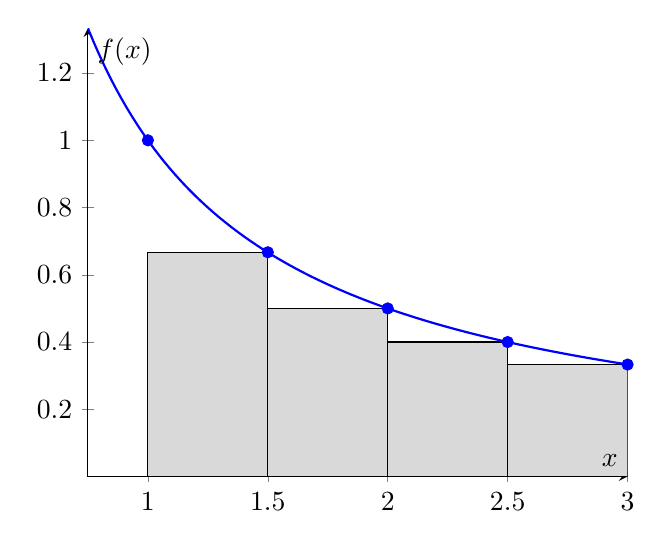
\begin{tikzpicture}
        \begin{axis}[axis lines = center, xmin=0.75, xmax=3, ymin=0, xlabel=$x$, ylabel=$f(x)$]
            \filldraw[fill=gray!30, draw=black] (1,0) rectangle (1.5,0.667);
            \filldraw[fill=gray!30, draw=black] (1.5,0) rectangle (2, 0.5);
            \filldraw[fill=gray!30, draw=black] (2,0) rectangle (2.5, 0.4);
            \filldraw[fill=gray!30, draw=black] (2.5,0) rectangle (3, 0.333);
            \addplot[blue, thick, samples=100, domain=0.75:3]{1/x};
            \addplot[mark=*, blue, only marks]coordinates{(1,1) (1.5,0.667) (2, 0.5) (2.5,.4) (3,0.333)};
        \end{axis}
    \end{tikzpicture}
    \caption{$R_4$ for $f(x)=\frac{1}{x}$}
    \label{fig:rightriemann}
\end{figure}

\subsection{Midpoint Riemann Sums}
A midpoint Riemann sum uses the value of $f(x)$ at the midpoint of the division to determine the height of the rectangle, as shown in figure \ref{fig:midriemann}. We will refer to the midpoint Riemann sum as $M_n$, where $n$ is the number of intervals. Then the total area approximated by the rectangles is $$M_n = f(\frac{x_0+x_1}{2})\Delta x + f(\frac{x_1+x_2}{x})\Delta x + \ldots + f(\frac{x_{n-1}+x_n}{2})\Delta x$$.

\begin{figure}
    \centering
    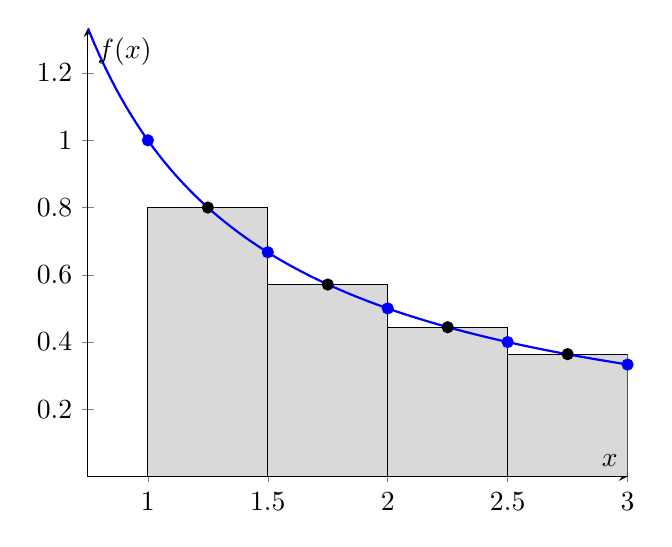
\begin{tikzpicture}
        \begin{axis}[axis lines = center, xmin=0.75, xmax=3, ymin=0, xlabel=$x$, ylabel=$f(x)$]
            \filldraw[fill=gray!30, draw=black] (1,0) rectangle (1.5,0.8);
            \filldraw[fill=gray!30, draw=black] (1.5,0) rectangle (2, 0.571);
            \filldraw[fill=gray!30, draw=black] (2,0) rectangle (2.5, 0.444);
            \filldraw[fill=gray!30, draw=black] (2.5,0) rectangle (3, 0.364);
            \addplot[blue, thick, samples=100, domain=0.75:3]{1/x};
            \addplot[mark=*, blue, only marks]coordinates{(1,1) (1.5,0.667) (2, 0.5) (2.5,.4) (3,0.333)};
            \addplot[mark=*, black, only marks]coordinates{(1.25,0.8) (1.75,0.571) (2.25, 0.444) (2.75,.364)};
        \end{axis}
    \end{tikzpicture}
    \caption{$M_4$ of $f(x)=\frac{1}{x}$}
    \label{fig:midriemann}
\end{figure}

\subsection{Additional Examples}
Sometimes we are working from real data and the intervals aren't evenly spaced. That's ok! We can still use Riemann sums to make an estimate. Consider the velocity data from the 1992 launch of the space shuttle \textit{Endeavour}, shown in tabular form in figure \ref{fig:endeavourdata}:

\begin{figure}
	\centering
	\begin{tabular}{c|c|c}
	Event & Time (s) & Velocity (ft/s) \\
	Launch & 0 & 0 \\
	Begin roll maneuver & 10 & 185 \\
	End roll maneuver & 15 & 319 \\
	Throttle to $89\%$ & 20 & 447 \\
	Throttle to $67\%$ & 32 & 742 \\
	Throttle to $104\%$ & 59 & 1325 \\
	Maximum dynamic pressure & 62 & 1445 \\
	Solid rocket booster separation & 125 & 4151 \\
	\end{tabular}
	\caption{Speed of \textit{Endeavour} from launch to booster separation}
	\label{fig:endeavourdata}
\end{figure}

We can use a Riemann sum to estimate how far the space shuttle traveled in the first 62 seconds of flight. First, let's visualize our data (see figure \ref{fig:endeavourscatter}). There are 7 time intervals from the data, but we only need the first 6. We can find a reasonable range for the distance the space shuttle travels by finding the left and right Riemann sums. Remember: because these data are strictly increasing, the left sum will be our lower bound and the right sum will be our upper bound. 

\begin{figure}
	\centering
	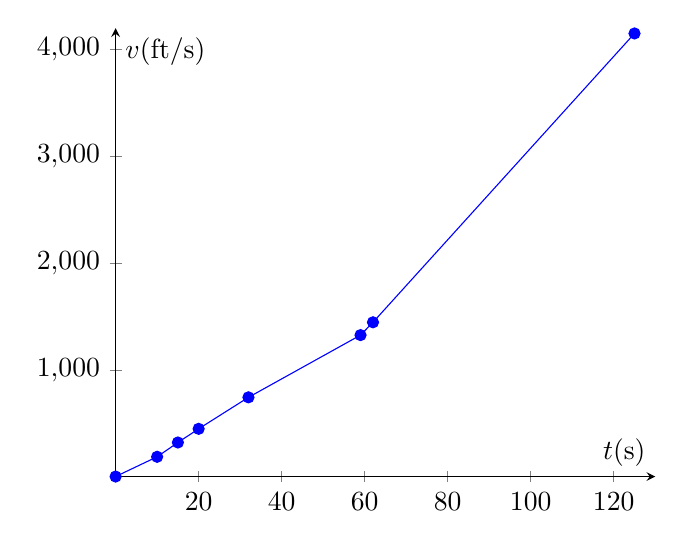
\begin{tikzpicture}
		\begin{axis}
		[axis lines = center,
		xlabel=$t$(s), 
		xmin=0,
		xmax=130,
		ylabel=$v$(ft/s),
		ymin=0,
		ymax=4200]
		\addplot[color=blue, mark=*]coordinates{(0,0) (10,185) (15, 319) (20, 447) (32, 742) (59, 1325) (62, 1445) (125, 4151)};
		\end{axis}
	\end{tikzpicture}
	\caption{Plot of time, velocity data for the \textit{Endeavour}}
	\label{fig:endeavourscatter}
\end{figure}

First, we'll find $L_6$. The width of the first interval is $10$ seconds ($10-0=10$) and the height of the rectangle will be $v(0) = 0$. Calculations for the additional intervals are shown in the table:
\begin{center}
\begin{tabular}{c|c|c|c}
	Interval & Width(s) & Height(ft/s) & Area(ft) \\
	1 & 10 & 0 & 0 \\
	2 & 5 & 185 & 925 \\
	3 & 5 & 319 & 1595 \\
	4 & 12 & 447 & 5364 \\
	5 & 27 & 742 & 20034 \\
	6 & 3 & 1325 & 3975 \\
\end{tabular}
\end{center}

Adding the areas, we find the lower limit for the distance traveled is 31,893 feet. We can determine the upper bound, $R_6$, in a similar manner:
\begin{center}
\begin{tabular}{c|c|c|c}
	Interval & Width(s) & Height(ft/s) & Area(ft) \\
	1 & 10 & 185 & 1850 \\
	2 & 5 & 319 & 1595 \\
	3 & 5 & 447 & 2235 \\
	4 & 12 & 742 & 8904 \\
	5 & 27 & 1325 & 35775 \\
	6 & 3 & 1445 & 4335 \\
\end{tabular}
\end{center}
Adding the areas, we find the upper limit for the distance traveled is 54,694 feet. Therefore, the \textit{Endeavour} traveled between 31,893 and 54,694 feet during the first 62 seconds of this flight. 

\section{Code for a Riemann Sum}
You can create a program that automatically calculates a Riemann sum. Create a file called riemann.py 
%\filname{riemann.py} FIXME \filname control sequence error
and type the following into it:

\begin{Verbatim}
import matplotlib.pyplot as plt
import sys
import math

from matplotlib.table import Rectangle

# Did the user supply two arguments?
if len(sys.argv) != 3:
    print(f"Usage: {sys.argv[0]} <stop> <divisions>")
    print(f"Numerically integrates 1/x from 1 to <stop>.")
    print(f"Calculates the value of 1/x at <divisions> spots in the range.")
    exit(1)

# Check to make sure the number of divisions is greater than zero?
divisions = int(sys.argv[2])
if divisions <= 0:
    print("ERROR: Divisions must be at least 1.")
    exit(1)

# Is the stopping point after 1.0?
stop = float(sys.argv[1])
if stop <= 1.0:
    print("ERROR: Stopping point must be greater than 1.0")
    exit(1)

start = 1.0
step_size = (stop - start)/divisions

print(f"Step size is {step_size:.5f}.")
x_values = []
y_values = []
sum = 0.0
for i in range(divisions):
    current_x = start + i * step_size
    current_y = 1.0/current_x
    area = current_y * step_size
    print(f"{i}: 1 / {current_x:.3f} = {current_y:4f}, area of rect = {area:8f} ")

    x_values.append(current_x)
    y_values.append(current_y)
    sum += area
    print(f"\tCumulative={sum:.3f}, ln({current_x:.3f})={math.log(current_x):.3f}")

print(f"Numerical integration of 1/x from 1.0 to {stop:.4f} is {sum:.4f}")
print(f"The natural log of {stop:.4f} is {math.log(stop):.4f}")

# Create data for the smooth 1/x line
SMOOTH_DIVISIONS = 200
smooth_start = start - 0.15
smooth_stop = stop + 1.0
smooth_step = (smooth_stop - smooth_start)/SMOOTH_DIVISIONS
smooth_x_values = []
smooth_y_values = []
for i in range(SMOOTH_DIVISIONS):
    current_x = smooth_start + i * smooth_step
    current_y = 1.0/current_x
    smooth_x_values.append(current_x)
    smooth_y_values.append(current_y)

# Put it on a plot
fig, ax = plt.subplots()
ax.set_xlim((smooth_x_values[0], smooth_x_values[-1]))
ax.set_ylim((0, smooth_y_values[0]))
ax.set_title("Riemann Sums for 1/x")

# Make the Riemann rects
for i in range(divisions):
    current_x = x_values[i]
    next_x = current_x + step_size
    current_y = y_values[i]
    rect = Rectangle((current_x, 0), step_size, current_y, edgecolor="green", facecolor="lightgreen")
    ax.add_patch(rect)

# Make the true 1/x curve
ax.plot(smooth_x_values, smooth_y_values, c="k", label="1/x")

# Show the user
plt.show()

\end{Verbatim}

This program will calculate and display a graph of the left Riemann sum of $\frac{1}{x}$ from 1 to the provided stop value with the indicated number of subintervals. When you run it, you'll see a graph in a new window and something like this in the terminal:
\begin{Verbatim}
Step size is 0.40000.
0: 1 / 1.000 = 1.000000, area of rect = 0.400000 
	Cumulative=0.400, ln(1.000)=0.000
1: 1 / 1.400 = 0.714286, area of rect = 0.285714 
	Cumulative=0.686, ln(1.400)=0.336
2: 1 / 1.800 = 0.555556, area of rect = 0.222222 
	Cumulative=0.908, ln(1.800)=0.588
3: 1 / 2.200 = 0.454545, area of rect = 0.181818 
	Cumulative=1.090, ln(2.200)=0.788
4: 1 / 2.600 = 0.384615, area of rect = 0.153846 
	Cumulative=1.244, ln(2.600)=0.956
5: 1 / 3.000 = 0.333333, area of rect = 0.133333 
	Cumulative=1.377, ln(3.000)=1.099
6: 1 / 3.400 = 0.294118, area of rect = 0.117647 
	Cumulative=1.495, ln(3.400)=1.224
7: 1 / 3.800 = 0.263158, area of rect = 0.105263 
	Cumulative=1.600, ln(3.800)=1.335
8: 1 / 4.200 = 0.238095, area of rect = 0.095238 
	Cumulative=1.695, ln(4.200)=1.435
9: 1 / 4.600 = 0.217391, area of rect = 0.086957 
	Cumulative=1.782, ln(4.600)=1.526
Numerical integration of 1/x from 1.0 to 5.0000 is 1.7820
The natural log of 5.0000 is 1.6094
\end{Verbatim}

\begin{Exercise}[label=rsumpython]
Use the python program you created to find $L_{10}$, $L_{50}$, $L_{100}$, $L_{500}$, $L_{1000}$, and $L_{5000}$ for the function $\frac{1}{x}$ from $x=1$ to $x=5$. What do you notice about the results?
\end{Exercise}

\begin{Answer}[ref=rsumpython]
	\begin{tabular}{c|c}
	Number of Intervals & Calculated Area\\
	10 & 1.7820 \\
	50 & 1.6419 \\
	100 & 1.6256 \\
	500 & 1.6126 \\
	1000 & 1.6110 \\
	5000 & 1.6098 \\
	\end{tabular}
	\\The area approaches the natural log of the endpoint, $\ln{5} \approx 1.6094$. 
\end{Answer}

\section{Riemann Sum Practice}

\begin{Exercise}[label=rsum2]
	\begin{center}
		\begin{tabular}{c|c|c|c|c}
			t (hours) & 4 & 7 & 12 & 15\\
			R(t) (L/hr) & 6.5 & 6.2 & 5.9 & 5.6\\
		\end{tabular}
	\end{center}
	A tank contains 50 liters of water after 4 hours of filling. Water is being added to the tank at rate $R(t)$. The value of $R(t)$ at select times is shown in the table. Using a right Riemann sum, estimate the amount of water in the tank after 15 hours of filling. 
\end{Exercise}

\begin{Answer}[ref=rsum2]
	The volume of water will be the amount of water at 4 hours (50 liters) plus the area under the graph of $R(t)$ from $t=4$ to $t=15$. We will estimate this area with a right Riemann sum. The approximate volume added from $t=4$ to $t=7$ is $(7-4)*(6.2) = 18.6$ liters. The approximate volume added from $t=7$ to $t=12$ is $(12-7)*(5.9)=29.5$ liters. The approximate volume added from $t=12$ to $t=15$ is $(15-12)*(5.6) = 16.8$ liters. Therefore, the approximate total volume of water in the tank at $t=15$ is $50 + 18.6 + 29.5 + 16.8 = 114.9$ liters. 
\end{Answer}

\begin{Exercise}[label=rsum3]
	Let $f(x) = x-2\ln{x}$. Estimate the area under $f$ from $x=1$ to $x=5$ using four rectangles and the value of $f$ at the midpoint of each interval. Sketch the curve and your approximating rectangles.
\end{Exercise}

\begin{Answer}[ref=rsum3]
	We will divide the area from $x=1$ to $x=5$ into four intervals at $x=2$, $x=3$, and $x=4$. Then we will find the value of $f(x)$ at the midpoint of each interval:
	\begin{center}
	\begin{tabular}{c|c|c}
	Interval & Midpoint & Value of $f(x)$ at midpoint\\
	1 & 1.5 & $\approx0.68907$\\
	2 & 2.5 & $\approx0.66742$\\
	3 & 3.5 & $\approx0.99447$\\
	4 & 4.5 & $\approx1.49185$\\
	\end{tabular}
\end{center}

Using the values in the table, we can make a possible sketch of $f(x)$:\\
	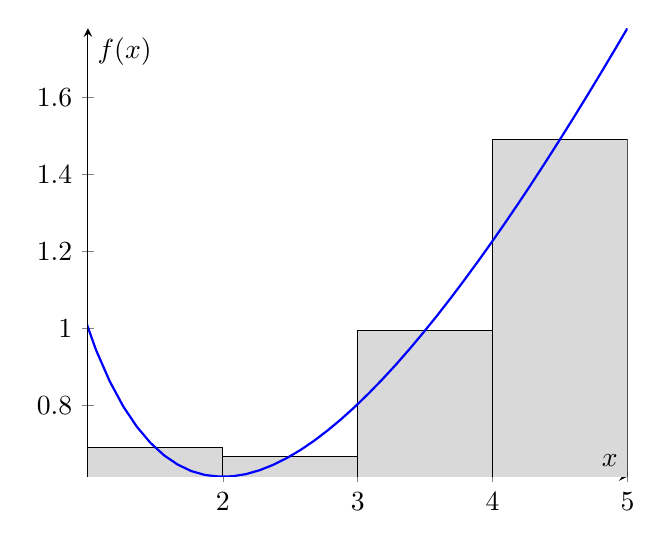
\begin{tikzpicture}
		\begin{axis}
		[axis lines = center, xmin=1, xmax=5, xlabel=$x$, ylabel=$f(x)$]
		\filldraw[fill=gray!30, draw=black](1,0) rectangle (2, 0.68907);
		\filldraw[fill=gray!30, draw=black](2, 0) rectangle (3, 0.66742);
		\filldraw[fill=gray!30, draw=black](3, 0) rectangle (4, 0.99447);
		\filldraw[fill=gray!30, draw=black](4, 0) rectangle (5, 1.49185);	
		\addplot[blue, thick, samples=100]{x-2*ln(x)};
		\end{axis}
	\end{tikzpicture}\\
	And we calculate the total area in the rectangles:
	$$1\times(0.68907+0.66742+0.99447+1.49185=3.84281$$
\end{Answer}

\begin{Exercise}[label=rsum4]
A graph of a car's velocity over a period of 60 seconds is shown. Estimate the distance traveled during this period. 
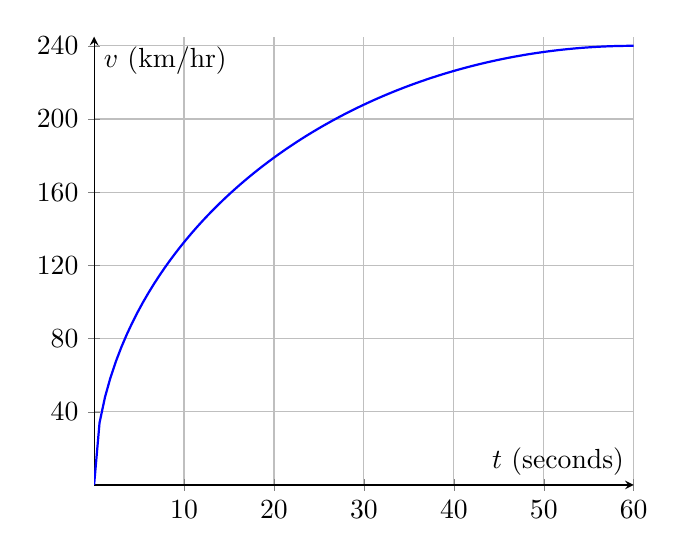
\begin{tikzpicture}
	\begin{axis}
	[axis lines = center, 
        xmin = 0, xmax = 60, xlabel=$t$ (seconds), 
        ymin=0, ymax=245, ylabel=$v$ (km/hr), ytick={40, 80, 120, 160, 200, 240}, xmajorgrids=true, ymajorgrids=true]
        \addplot[blue, thick, samples=100, domain=0:60]{4*sqrt(3600-(x-60)^2)};
	\end{axis}
\end{tikzpicture}
\end{Exercise}

\begin{Answer}[ref=rsum4]
The question allows the student to choose the type of sum (left, right, or midpoint) and the number of intervals. A possible solution is given, but there are many ways to answer the question.\\
The tricky part here is noticing the units! In order to have a solution in kilometers, we'll need to convert km/hr to m/s when we calculate the areas. A possible solution is to divide the graph into 6 intervals (one every 10 seconds) and use a right Riemann sum.

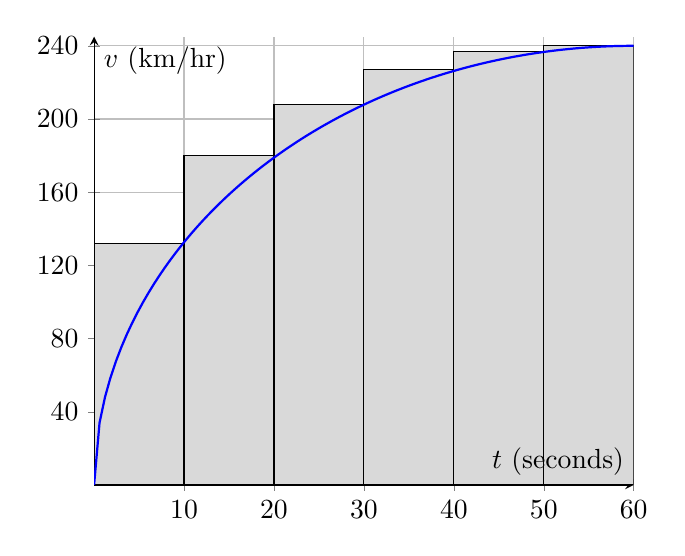
\begin{tikzpicture}
	\begin{axis}
	[axis lines = center, 
        xmin = 0, xmax = 60, xlabel=$t$ (seconds), 
        ymin=0, ymax=245, ylabel=$v$ (km/hr), ytick={40, 80, 120, 160, 200, 240}, xmajorgrids=true, ymajorgrids=true]
        \filldraw[fill=gray!30, draw=black](0,0) rectangle (10,132);
        \filldraw[fill=gray!30, draw=black](10, 0) rectangle (20, 180);
        \filldraw[fill=gray!30, draw=black](20, 0) rectangle (30, 208);
        \filldraw[fill=gray!30, draw=black](30, 0) rectangle (40, 227);
        \filldraw[fill=gray!30, draw=black](40, 0) rectangle (50, 237);
        \filldraw[fill=gray!30, draw=black](50, 0) rectangle (60, 240);
        \addplot[blue, thick, samples=100, domain=0:60]{4*sqrt(3600-(x-60)^2)};
	\end{axis}
\end{tikzpicture}\\
We can use the graph to \textit{estimate} the height of each rectangle. Some reasonable estimates are $f(10) = 130\frac{km}{hr}\approx36.1\frac{ms}{s}$, $f(20) = 180\frac{km}{hr}=50\frac{m}{s}$, $f(30) = 210\frac{km}{hr}\approx58.3\frac{m}{s}$, $f(40) = 230\frac{km}{hr}\approx63.9\frac{m}{s}$, $f(50) = 235\frac{km}{hr}\approx65.3\frac{m}{s}$, and $f(60) = 240\frac{km}{hr}\approx66.7\frac{m}{s}$. [Any values within $\pm5$ of the listed values are reasonable.] Noting that each interval is $10$ sec wide and using the estimates of $f(x)$ listed, we can estimate that the distance traveled is $10\text{ }sec\times(36.1\frac{m}{s}+50\frac{m}{s}+58.3\frac{m}{s}+63.9\frac{m}{s}+65.3\frac{m}{s}+66.7\frac{m}{s})=3403$ meters.
\end{Answer}